\chapter{Ejercicio 2}

\section{Actividad 1}

\subsection{A}

\textbf{A)} Expresar la Ecuación Diferencial (ED) que describe el circuito, y con ello, definir un
Sistema en tiempo continuo con entrada x(t) = v(t) y salida y(t) = i(t) , con condiciones
Iniciales genérica (CI).

\begin{figure}[H]
  \centering
  \begin{circuitikz}[american voltages]
    \node at (-3,1) {ENTRADA};
    \node at (-3,0) {$x(t) = v(t)$};
    
    \draw (-1,-1) rectangle (3.5,2.5);

    \draw (-0.5,1.5) to[R=$R$] (2,1.5)
          to[C=$C$] (2,-0.5) -- (-0.5,-0.5);
    
    \draw[->] (-4, 0.5) -- (-1,0.5);

    \node at (6,1) {SALIDA};
    \node at (6,0) {$y(t) = i(t)$};
    
    \draw[->] (3.5,0.5) -- (6,0.5);
  \end{circuitikz}
\end{figure}

Para plantear la EDO es necesario plantear ley de kirchoff

$$v(t) = R \cdot i(t) + \dfrac{1}{C} \cdot \int i(t) dt$$

Ahora derivamos para conseguir la expresion buscada

$$\dfrac{d v(t)}{dt} = R \dfrac{d i(t)}{dt} + \dfrac{1}{C} \cdot i(t)$$

Dividimos todo por $R$ para normalizar la ecuacion

$$\dfrac{d i(t)}{dt} + \dfrac{1}{RC} \cdot i(t) = \dfrac{1}{R} \cdot \dfrac{d v(t)}{dt}$$

$$y'(t) + \dfrac{1}{RC} \cdot y(t) = \dfrac{1}{R} \cdot x'(t)$$

Para el circuito de segundo orden:

\begin{figure}[H]
  \centering
  \begin{circuitikz}[american voltages]
    \node at (-3,1) {ENTRADA};
    \node at (-3,0) {$x(t) = v(t)$};
    
    \draw (-1,-1) rectangle (3.5,2.5);

    \draw (-0.5,1.5) to[R=$R$] (1.25,1.5) to[L=$L$] (2.3,1.5)
          to[C=$C$] (2.3,-0.5) -- (-0.5,-0.5);
    
    \draw[->] (-4, 0.5) -- (-1,0.5);

    \node at (6,1) {SALIDA};
    \node at (6,0) {$y(t) = i(t)$};
    
    \draw[->] (4,0.5) -- (6,0.5);
  \end{circuitikz}
\end{figure}

Siguiendo con el mismo procedimiento

$$v(t) = R \cdot i(t) + L \cdot \dfrac{d i(t)}{dt} + \dfrac{1}{C} \cdot \int i(t) dt$$

$$\dfrac{d v(t)}{dt} = R \cdot \dfrac{d i(t)}{dt} + L \cdot \dfrac{d^2 i(t)}{dt^2} + \dfrac{1}{C} \cdot i(t)$$

$$\dfrac{d^2 i(t)}{dt^2} +  \dfrac{R}{L} \cdot \dfrac{d i(t)}{dt} + \dfrac{1}{LC} \cdot i(t) = \dfrac{1}{L} \cdot \dfrac{d v(t)}{dt} $$

$$y''(t) + \dfrac{R}{L} \cdot y'(t) + \dfrac{1}{LC} \cdot y(t) = \dfrac{1}{L} \cdot x'$$

\subsection{B}

\textbf{B)}Usar la transformada de Laplace para sintetizar el sistema en la expresión

Primero sintetizamos la ecuacion correspondiente al circuito de primer orden

$$\mathscr{L}[y'(t)] = sY(s) - y(0)$$

$$\mathscr{L}[y(t)] = Y(s)$$

$$\mathscr{L}[x'(t)] = sX(s) - x(0)$$

Quedando la ecuacion

$$sY(s) - y(0) + \dfrac{1}{RC} \cdot Y(s) = \dfrac{1}{R} \cdot (sX(s) - x(0))$$

$$Y(s) (s + \dfrac{1}{rc}) = \dfrac{1}{R} \cdot sX(s) - \dfrac{1}{R} x(0) + y(0)$$

$$Y(s) = X(s)  \dfrac{\dfrac{s}{R}}{s + \dfrac {1}{RC}} + \dfrac{1}{(s + \dfrac{1}{RC})} [y(0) - x(0) \dfrac{1}{R}]$$

Ya nos queda sintetizado a la expresion

$$Y(s) = X(s) \cdot H(s) + F(s,CI)$$

Ahora para el circuito de segundo orden, primero debemos definir la transformada para la segunda derivada

$$\mathscr{L}[y''(t)] = s^2Y(s) - sy(0) - y'(0)$$

Quedando la ecuacion sintetizada

$$ s^2Y(s) - s y(0) - y'(0) + \dfrac{R}{L} (sY(s) - y(0)) + \dfrac{1}{LC} \cdot Y(s) = \dfrac{1}{L} \cdot (sX(s) - x(0))$$

$$ Y(s) (s^2 + \dfrac{R}{L} s + \dfrac{1}{LC}) = X(s) \dfrac{s}{L} - x(0) \dfrac{1}{L} + s y(0) + y'(0) + \dfrac{R}{L} y(0)$$

$$ Y(s) = X(s) \dfrac{\dfrac{s}{L}}{s^2 + \dfrac{R}{L} s + \dfrac{1}{LC}} + \dfrac{1}{s^2 + \dfrac{R}{L} s + \dfrac{1}{LC}} [s y(0) + y'(0) + \dfrac{R}{L} y(0) - x(0) \dfrac{1}{L}]$$

\subsection{C}

\textbf{C)} Escribir un diagrama de Bloques en la variable compleja S que determine al Sistema.

El diagrama de bloques que describe a la ecuacion de primer orden es:

\begin{figure}[H]
  \centering
  \begin{circuitikz}
    \node at (-2.5,1) {$X(s)$};
    \draw[->] (-3,0.5) -- (0,0.5);

    \draw (0,1) rectangle (1,0);

    \node at (0.5,0.5) {$H(s)$};
  
    \draw (1,0.5) -- (3,0.5);
    \draw[->] (3,0.5) -- (3,-0.5);

    \node at (-2.5,-2) {$F(s,CI)$};
    \draw[->] (-3,-2.5) -- (0,-2.5);

    \draw (0,-1.87) rectangle (1.25,-3.12);
    
    \draw (1.25,-2.5) -- (3,-2.5);
    \draw[->] (3,-2.5) -- (3,-1);

    \node[scale=0.7] at (0.625,-2.475) {$\dfrac{1}{s+\dfrac{1}{RC}}$};

    \draw (3,-0.75) circle (0.25cm);

    \node at (3,-0.75) {+};

    \draw[->] (3.25,-0.75) -- (4.25,-0.75);
    \node at (4,-0.25) {$Y(s)$};
  \end{circuitikz}
\end{figure}

Por otro lado el que describe a la ecuacion de segundo orden

\begin{figure}[H]
  \centering
  \begin{circuitikz}
    \node at (-2.5,1) {$X(s)$};
    \draw[->] (-3,0.5) -- (0,0.5);

    \draw (0,1) rectangle (1,0);

    \node at (0.5,0.5) {$H(s)$};
  
    \draw (1,0.5) -- (3,0.5);
    \draw[->] (3,0.5) -- (3,-0.5);

    \node at (-2.5,-2) {$F(s,CI)$};
    \draw[->] (-3,-2.5) -- (0,-2.5);

    \draw (0,-1.87) rectangle (1.25,-3.12);
    
    \draw (1.25,-2.5) -- (3,-2.5);
    \draw[->] (3,-2.5) -- (3,-1);

    \node[scale=0.45] at (0.625,-2.475) {$\dfrac{\dfrac{s}{L}}{s^2+\dfrac{R}{L}s+\dfrac{1}{LC}}$};

    \draw (3,-0.75) circle (0.25cm);

    \node at (3,-0.75) {+};

    \draw[->] (3.25,-0.75) -- (4.25,-0.75);
    \node at (4,-0.25) {$Y(s)$};
  \end{circuitikz}
\end{figure}

\subsection{D}

\textbf{D)} Graficar en el plano $S$ polos y ceros de $H(s)$.

Para el caso de primer orden

$$H(s) = \dfrac{\dfrac{s}{R}}{s + \dfrac{1}{RC}}$$

Donde el unico polo se encuentra en $s=-\dfrac{1}{RC}$ y el cero en $s=0$.

$R = 3$, $C = \dfrac{1}{2}$, $L = 1$.

El polo con estos datos seria $s=-\dfrac{2}{3}$

\begin{figure}[H]
  \centering
  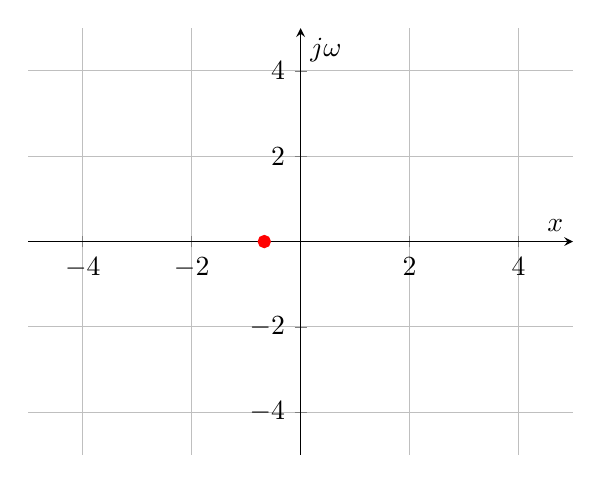
\begin{tikzpicture}
    \begin{axis}[
        axis lines=middle,
        xlabel={$x$},
        ylabel={$j\omega$},  
        grid=both,
        width=8.5cm,
        height=7cm,
        ymin=-5, ymax=5,
        xmin=-5, xmax=5,
      ]
      \addplot[red, thick, mark=*] coordinates {(-2/3,0)};
    \end{axis}
  \end{tikzpicture}
\end{figure}

Para la ecuacion de segundo orden 

$$H(s) = \dfrac{\dfrac{s}{L}}{s^2 + \dfrac{R}{L} s + \dfrac{1}{LC}}$$

Y los polos se encontrarian en $s_n=\dfrac{-\dfrac{R}{L} \pm \sqrt{\dfrac{R}{L}^2-\dfrac{4}{LC}}}{2}$

Donde reemplazando con los valores previamente dados, los polos quedarian en $(-1,0)$ y $(-2,0)$.

\begin{figure}[H]
  \centering
  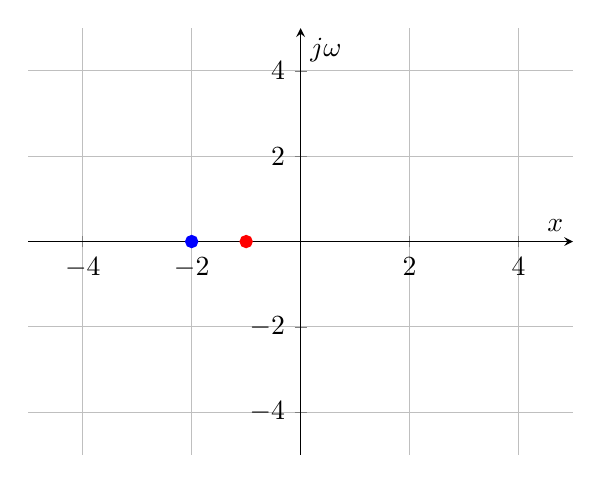
\begin{tikzpicture}
    \begin{axis}[
        axis lines=middle,
        xlabel={$x$},
        ylabel={$j\omega$},  
        grid=both,
        width=8.5cm,
        height=7cm,
        ymin=-5, ymax=5,
        xmin=-5, xmax=5,
      ]
      \addplot[red, thick, mark=*] coordinates {(-1,0)};
      \addplot[blue, thick, mark=*] coordinates{(-2,0)};
    \end{axis}
  \end{tikzpicture}
\end{figure}

\subsection{E}

\textbf{E)} Obtener la respuesta al impulso, $h(t)$, suponiendo que las CI = 0.

Continuaremos resolviendo primero la ecuacion de primer orden

$$\mathscr{L} [\delta (t)] = 1$$

$$\mathscr{L}^{-1} [H(s) \cdot 1] = \mathscr{L} [H(s)]$$

$$H(s) = \dfrac{1}{R} \dfrac{s}{s + \dfrac{1}{RC}}$$

$$\dfrac{1}{RC} = a$$

$$H(s) = \dfrac{1}{R} \dfrac{s + a - a}{s + a}$$

$$H(s) = \dfrac{1}{R} (\dfrac{s + a}{s + a} - \dfrac{a}{s + a})$$

$$H(s) = \dfrac{1}{R} (1 - \dfrac{a}{s + a})$$

$$h(t) = \mathscr{L}^{-1} [\dfrac{1}{R} (1 - \dfrac{a}{s + a})] = \dfrac{1}{R} \mathscr{L}^{-1} [1 - \dfrac{a}{s + a}] = \dfrac{1}{R} (\mathscr{L}^{-1} [1] - \mathscr{L}^{-1} [\dfrac{a}{s + a}])$$

$$\mathscr{L}^{-1} [1] = \delta (t) $$

$$\mathscr{L}^{-1} [\dfrac{a}{s + a}] = a e^{-at} u(t)$$

$$h(t) = \dfrac {1}{R} (\delta (t) - a e^{at} u(t))$$

$$h(t) = \dfrac {1}{R} (\delta (t) - \dfrac{1}{RC} e^{\dfrac{1}{RC} t} u(t))$$

$$h(t) = \dfrac{\delta (t)}{3} - \dfrac{2}{9} e^{\frac{2}{3}} u(t)$$

Para la ecuacion de segundo orden

$$H(s) = \dfrac{\dfrac{s}{L}}{s^2 + \dfrac{R}{L} s + \dfrac{1}{LC}}$$

$$\dfrac{R}{L} = a; \dfrac{1}{LC} = b$$

$$H(s) = \dfrac{1}{L} \dfrac{s}{s^2 + a s + b}$$

$$H(s) = \dfrac{1}{L} \dfrac{s}{(s + 1) (s + 2)}$$

$$H(s) = \dfrac{1}{L} \frac{-1}{s + 1} + \frac{2}{s + 2} $$

$$h(t) = \mathscr{L}^{-1} [H(s)] = \mathscr{L}^{-1} [\frac{1}{L} \frac{-1}{s + 1} + \frac{2}{s + 2}]$$

$$h(t) = \frac{1}{L} \mathscr{L}^{-1} [\frac{-1}{s + 1} + \frac{2}{s + 2}]$$

$$h(t) = \frac{1}{L} (-\mathscr{L}^{-1} (\frac{1}{s + 1}) + \mathscr{L}^{-1} (\frac{2}{s + 2}))$$

$$h(t) = \frac{1}{L} (-e^{-t} u(t) + 2 e^{-2t} u(t))$$

$$h(t) = \frac{1}{L} u(t) (-e^{-t} + 2 e^{-2t})$$

\subsection{F}

\textbf{F)} Obtener la respuesta al escalón unitario $v(t)$, suponiendo CI = 0 y verificar la identidad $\frac{d}{dt} v(t) = h(t), \forall t$

Para la ecuacion de primer orden

$$v(t) = \mathscr{L}^{-1} (H(s) \cdot \mathscr{L} (u(t)))$$

$$v(t) = \mathscr{L}^{-1} (\dfrac{\dfrac{s}{R}}{s + \dfrac{1}{RC}} \cdot \dfrac{1}{s})$$

$$v(t) = \dfrac{1}{R} \mathscr{L}^{-1} (\dfrac{1}{s + \dfrac{1}{RC}})$$

$$\dfrac{1}{RC} = a $$

$$v(t) = \dfrac{1}{R} \mathscr{L}^{-1} (\dfrac{1}{s + a}) $$

$$v(t) = \dfrac{1}{R} e^{-at} u(t) $$

$$v(t) = \dfrac{1}{3} e^{-\dfrac{2}{3}t} u(t)$$

En el caso de la ecuacion de segundo orden

$$v(t) = \mathscr{L}^{-1} (\dfrac{\dfrac{s}{L}}{s (s + 1) (s + 2)})$$

$$v(t) = \dfrac{1}{L} \mathscr{L}^{-1} (\dfrac{1}{(s + 1)(s + 2)})$$

Por fracciones simples

$$v(t) = \dfrac{1}{L} \mathscr{L}^{-1} (\dfrac{A}{s + 1} \dfrac{B}{s + 2})$$

$$v(t) = \dfrac{1}{L} \mathscr{L}^{-1} (\dfrac{1}{s + 1} - \dfrac{1}{s + 2})$$

$$v(t) = \dfrac{1}{L} \mathscr{L}^{-1} (\dfrac{1}{s + 1}) - \mathscr{L}^{-1} (\dfrac{1}{s + 2})$$

$$v(t) = \dfrac{1}{L} (e^{-t} - e^{-2t}) u(t) $$

$$L=1$$

$$v(t) = (e^{-t} - e ^{-2t}) u(t)$$

Ahora para ambos casos vamos a verificar que $\dfrac{dv(t)}{dt} = h(t)$

En ambos casos vamos a usar que $\dfrac{d}{dt} [f(t)u(t)] = f(0)\delta (t) + f'(t) u(t)$, siendo para el la ecuacion de primer orden

$$v(0) = \dfrac{1}{3} $$

$$v'(t) = \dfrac{-2}{9} e^{-\dfrac{2}{3}}$$

Quedando

$$\dfrac{dv(t)}{dt} = \dfrac{\delta(t)}{3} - \dfrac{2}{9} e^{-\dfrac{2}{3}} u(t) $$

Por lo cual se verifica para la primera ecuacion, por otro lado para la segunda ecuacion

$$v(0) = e^{-0} - e^{0} = 1 - 1 = 0$$

$$v'(t) = e^{-t} + 2e^{-2t} $$

Lo cual aplicando lo explicado anteriormente

$$\dfrac{dv(t)}{dt} = 0 \delta(t) + e^{-t} + 2e^{-2t} u(t) $$

$$\dfrac{dv(t)}{dt} = e^{-t} + 2e^{-2t} u(t) = h(t)$$

\subsection{G}

\textbf{G)} Obtener la respuesta a la rampa.

Primero transformamos la integral del escalon

$$\mathscr{L} (\int_{-\infty}^{t} u(\tau) d\tau)$$

$$\mathscr{L} (\int_{-\infty}^{0} 0 d\tau + \int_{0}{t} 1 d\tau)$$

$$\mathscr{L} (t)$$

$$\mathscr{L} (t) = \dfrac{1}{s^2}$$

Entonces para calcular la respuesta a la rampa con la ecuacion de primer orden

$$y(t) = \mathscr{L}^{-1} (H(s)\dfrac{1}{s^2})$$

$$y(t) = \mathscr{L}^{-1} (\dfrac{\dfrac{s}{R}}{s + \dfrac{1}{RC}} \cdot \dfrac{1}{s^2})$$

$$y(t) = \dfrac{1}{R} \mathscr{L}^{-1} (\dfrac{1}{s(s + \dfrac{1}{RC})})$$

$$\dfrac{1}{RC} = \dfrac{2}{3} = a$$

$$y(t) = \dfrac{1}{R} \mathscr{L}^{-1} (\dfrac{A}{s} + \dfrac{B}{s + a}) $$

$$A=\dfrac{1}{a}; B=-\dfrac{1}{a} $$

$$y(t) = \dfrac{1}{R} \dfrac{1}{a} \mathscr{L}^{-1}(\dfrac{1}{s} - \dfrac{1}{s+a}) $$

$$y(t) = \dfrac{1}{R} \dfrac{1}{a} (\mathscr{L}^{-1}\dfrac{1}{s} - \mathscr{L}^{-1}\dfrac{1}{s+a})$$

$$y(t) = \dfrac{1}{R} \dfrac{1}{a} (u(t) - e^{-at}u(t))$$

$$y(t) = \dfrac{1}{aR} u(t) (1 - e^{-at})$$

$$y(t) = C u(t) (1 - e^{-\dfrac{1}{RC}t}) $$

$$y(t) = \dfrac{1}{2} u(t) (1 - e^{-\dfrac{2}{3}t}) $$

Para el caso de la ecuacion de segundo orden, recordamos que

$$H(s) = \dfrac{\dfrac{s}{L}}{s^2 + \dfrac{R}{L} s + \dfrac{1}{LC}}$$

$$y(t) = \mathscr{L}^{-1} (\dfrac{\dfrac{s}{L}}{s^2 + \dfrac{R}{L} s + \dfrac{1}{LC}} \cdot \dfrac{1}{s^2})$$

$$y(t) = \dfrac{1}{L} \mathscr{L}^{-1} (\dfrac{1}{s(s^2 + \dfrac{R}{L} s + \dfrac{1}{LC})}) $$

$$y(t) = \dfrac{1}{L} \mathscr{L}^{-1} (\dfrac{1}{s(s+1)(s+2)}) $$

$$y(t) = \dfrac{1}{L} \mathscr{L}^{-1} (\dfrac{A}{s} + \dfrac{B}{s+1} + \dfrac{C}{s+2})$$

$$y(t) = \dfrac{1}{L} \mathscr{L}^{-1} (\dfrac{\dfrac{1}{2}}{s} - \dfrac{1}{s+1} + \dfrac{\dfrac{1}{2}}{s+2}) $$

$$y(t) = \dfrac{1}{L} [\dfrac{1}{2} \mathscr{L}^{-1} (\dfrac{1}{s}) - \mathscr{L}^{-1} (\dfrac{1}{s+1}) + \dfrac{1}{2} \mathscr{L}^{-1} (\dfrac{1}{s+2})] $$

$$y(t) = \dfrac{1}{L} [\dfrac{1}{2} u(t) - e^{-t} u(t) + \dfrac{1}{2} e^{-2t} u(t)] $$

$$y(t) = \dfrac{1}{L} u(t) [\dfrac{1}{2} - e^{-t} + \dfrac{e^{-2t}}{2}]$$

$L = 1$

$$y(t) = u(t) [\dfrac{1}{2} - e^{-t} + \dfrac{e^{-2t}}{2}] $$

Vamos a completar este ejercicio realizando al verificacion de los calculos mediante la siguiente igualdad $y(t) = \int_{-\infty}^{t} v(\tau) d\tau$.

Manteniendo el orden de realizacion de ejercicios, comenzamos con la ecuacion de primer orden

$$v(t) = \dfrac{1}{3} e^{-\dfrac{2}{3}t} u(t)$$

$$\int_{-infty}^{t} v(t) = \dfrac{1}{3} \int_{0}^{t} e^{-\dfrac{2}{3}\tau} d\tau = y(t) $$

$a = \dfrac{-2}{3}$

$$y(t) = \dfrac{1}{3} [\dfrac{1}{a} e^{at} \bigg\rvert_{0}^{t}] $$

$$y(t) = \dfrac{1}{3} \dfrac{1}{a} (e^{at} - 1) $$

$$y(t) = -\dfrac{1}{2} e^{-\dfrac{2}{3}t} - \dfrac{1}{2} $$

$$y(t) = \dfrac{1}{2} (1 - e^{-\dfrac{2}{3}t}) $$ 

Verificando correctamente para la primera ecuacion, ahora correspondemos con la de segundo orden

$$v(t) = (e^{-t} - e^{-2t}) u(t) $$

$$\int_{-\infty}^{t} v(t) = y(t) $$

$$\int_{-\infty}^{t} v(t) = \int_{0}^{t} (e^{-\tau} - e^{-2\tau}) d\tau $$

$$\int_{-\infty}^{t} v(t) = \int_{0}^{t} e^-{-\tau} d\tau - \int_{0}^{t} e^{-2\tau} d\tau $$ 

$$\int_{-\infty}^{t} v(t) = -e^{-\tau}\bigg\rvert_{0}^{t} - (-\dfrac{1}{2} e^{-2\tau} \bigg\rvert_{0}^{t}) $$

$$\int_{-\infty}^{t} v(t) = -(e^{-t} - 1) - (-\dfrac{1}{2} e^{-2t} + \dfrac{1}{2}) $$

$$\int_{-\infty}^{t} v(t) = 1 - e^{-t} + \dfrac{1}{2} e^{-2t} - \dfrac{1}{2}$$

$$\int_{-\infty}^{t} v(t) = \dfrac{1}{2} - e^{-t} + \dfrac{1}{2} e^{-2t}$$

Su forma causal

$$\int_{-\infty}^{t} v(t) = u(t) [\dfrac{1}{2} - e^{-2t} + \dfrac{1}{2} e^{-2t}]$$

Por lo cual se verifica todo lo calculado anteriormente.

\section{Actividad 2}

\subsection{A}

\textbf{Circuito RC}

De la Ley de Voltajes de Kirchhoff y la relación del capacitor:

\[
v(t) = R i(t) + v_C(t), 
\qquad 
i(t) = C \, v_C'(t) 
\;\;\;\Rightarrow\;\;\;
v_C'(t) = \frac{1}{C} y(t).
\]

La ecuación diferencial queda:
\[
y'(t) + \frac{1}{RC}\,y(t) = \frac{1}{R}\,x'(t)
\]

\[
  D y(t) + \dfrac{1}{RC} \, y(t) = \dfrac{1}{R} D x(t)
\]

\[
  y(t) = \dfrac{1}{R} \, x(t) - D^{-1} \bigg( \dfrac{1}{RC} \, y(t)\bigg)
\]

\begin{figure}[H]
  \centering
  \begin{circuitikz}
    \node at (0,0) {$x(t)$};

    \draw (0.5,0) -- (2.5,0);
    \draw[->] (2.5,0) -- (2.5,-1);

    \draw (2,-1) rectangle (3,-2);

    \node at (2.5, -1.5) {$\dfrac{1}{R}$};

    \draw[->] (2.5,-2) -- (2.5,-2.5);\

    \draw (2.5,-2.75) circle (0.25cm);

    \node at (2.5, -2.75) {$-$};

    \draw (2.75, -2.75) -- (4, -2.75);

    \draw[->] (4,-2.75) -- (5, -2.75);
    \node at (5, -2.3) {$y(t)$};

    \draw (4, -2.75) -- (4, -4);
    \draw[->] (4, -4) -- (3, -4);

    \draw (2, -3.5) rectangle (3, -4.5);

    \node[scale=0.8] at (2.5, -4) {$\dfrac{1}{RC}$};

    \draw (2, -4) -- (0, -4);
    \draw (0, -4) -- (0, -2.75);
    \draw[->] (0,-2.75) -- (1, -2.75);

    \draw (1,-2.25) rectangle (2, -3.25);

    \node at (1.5, -2.75) {$\int$};

    \draw[->] (2, -2.75) -- (2.25, -2.75);
  \end{circuitikz}
\end{figure}

\textbf{Circuito RLC}

De la Ley de Voltajes de Kirchhoff y la relación de los elementos (RLC):

\[
x(t) = R\,i(t) + L\,i'(t) + v_C(t),
\qquad 
i(t) = C\,v_C'(t).
\]

La ecuación diferencial queda:
\[
y''(t) + \frac{R}{L}\,y'(t) + \frac{1}{LC}\,y(t) = \frac{1}{L}\,x'(t).
\]

$$D^2 y(t) + D\bigg[\dfrac{R}{L} \, y(t)\bigg] + \dfrac{1}{LC} y(t) = D \bigg[\dfrac{1}{L} x(t)\bigg]$$

$$D^2 y(t) = D \bigg[\dfrac{1}{L} \, x(t) - \dfrac{R}{L} \, y(t)\bigg] - \dfrac{1}{LC} y(t) $$

$$y(t) = D^{-1} \bigg[\dfrac{1}{L} \, x(t) - \dfrac{R}{L} \, y(t)\bigg] - D^{-2} \dfrac{1}{LC} y(t)$$

$$y(t) = D^{-1} \bigg[\dfrac{1}{L} \, x(t) - \dfrac{R}{L} \, y(t) - D^{-1} \bigg(\dfrac{1}{LC} y(t) \bigg)  \bigg] $$

\begin{figure}[H]
  \centering
  \begin{circuitikz}
    \node at (0,0) {$x(t)$};

    \draw (0.5,0) -- (2.5,0);
    \draw[->] (2.5,0) -- (2.5,-1);

    \draw (2,-1) rectangle (3,-2);

    \node at (2.5, -1.5) {$\dfrac{1}{L}$};

    \draw[->] (2.5,-2) -- (2.5,-2.5);

    \draw (2.5,-2.75) circle (0.25cm);

    \node at (2.5, -2.75) {$-$};

    \draw (2.75, -2.75) -- (3.25, -2.75);

    \draw (3.25, -2.25) rectangle (4.25, -3.25);

    \node at (3.75, -2.75) {$\int$};

    \draw (4.25, -2.75) -- (5, -2.75);

    \draw[->] (5,-2.75) -- (5.5, -2.75);
    \node at (5.5, -2.3) {$y(t)$};

    \draw (5, -2.75) -- (5, -5);
    \draw (5, -5) -- (0, -5);
    \draw[->] (2.5, -5) -- (2.5, -4.5);

    \draw (2, -3.5) rectangle (3, -4.5);

    \node at (2.5, -4) {$\dfrac{R}{L}$};

    \draw[->] (2.5, -3.5) -- (2.5,-3);

    \draw[->] (0, -5) -- (0, -4.5);

    \draw (-0.5, -3.5) rectangle (0.5, -4.5);

    \node at (0, -4) {$\dfrac{1}{LC}$};

    \draw (0, -3.5) -- (0, -2.75);
    \draw[->] (0,-2.75) -- (1,-2.75);

    \draw (1,-2.25) rectangle (2, -3.25);

    \node at (1.5, -2.75) {$\int$};

    \draw[->] (2, -2.75) -- (2.25, -2.75);
  \end{circuitikz}
\end{figure}


% ------------------------------------------------------------
\subsection{B}

\textbf{Circuito RC}

\textbf{Función de transferencia e impulso}

\[
H(s) = \frac{\tfrac{s}{R}}{s+\tfrac{1}{RC}}.
\]

\[
h(t) = \mathscr{L}^{-1}\{H(s)\} 
= \frac{1}{R}\Big[\delta(t)-\frac{1}{RC}e^{-t/(RC)}u(t)\Big].
\]

\textbf{Respuesta al escalón}

Entrada:
\[
x(t)=u(t), \quad X(s)=\frac{1}{s}.
\]

\[
Y(s) = H(s)\,X(s) 
= \frac{\tfrac{s}{R}}{s+\tfrac{1}{RC}} \cdot \frac{1}{s}
= \frac{1}{R}\cdot \frac{1}{s+\tfrac{1}{RC}}.
\]

\[
y(t) = \frac{1}{R}\,e^{-t/(RC)}u(t).
\]

Verificación con convolución en tiempo:

\begin{align*}
v(t) &= \int_{0}^{t} h(\tau)\,d\tau \\
     &= \frac{1}{R}\left( \int_{0}^{t}\delta(\tau)\,d\tau 
     - \frac{1}{RC}\int_{0}^{t} e^{-\tau/(RC)}\,d\tau \right) \\
     &= \frac{1}{R}\left(1 - \big(1-e^{-t/(RC)}\big)\right) \\
     &= \frac{1}{R}\,e^{-t/(RC)}u(t).
\end{align*}

\textbf{Respuesta a la rampa}

Entrada:
\[
x(t)=t\,u(t), \quad X(s)=\frac{1}{s^2}.
\]

\[
Y(s) = H(s)\,X(s) 
= \frac{\tfrac{s}{R}}{s+\tfrac{1}{RC}} \cdot \frac{1}{s^2}
= \frac{1}{R}\,\frac{1}{s(s+\tfrac{1}{RC})}.
\]

Descomposición en fracciones simples:
\[
\frac{1}{s(s+\tfrac{1}{RC})} = \frac{RC}{s} - \frac{RC}{s+\tfrac{1}{RC}}.
\]

\[
Y(s)=\frac{1}{R}\left(\frac{RC}{s}-\frac{RC}{s+\tfrac{1}{RC}}\right).
\]

\[
y(t) = C\big(1-e^{-t/(RC)}\big)u(t).
\]

% ------------------------------------------------------------
\textbf{Ciruito RLC}

\textbf{Función de transferencia e impulso}

\[
H(s) = \frac{\tfrac{s}{L}}{s^2+\tfrac{R}{L}s+\tfrac{1}{LC}}
= \frac{1}{L}\,\frac{s}{(s-s_1)(s-s_2)}
\]

Con

\[
s_{1,2} = \frac{-\tfrac{R}{L}\pm \sqrt{\left(\tfrac{R}{L}\right)^2-\tfrac{4}{LC}}}{2} ; 
\quad s_1 \neq s_2
\]

Descomposición en fracciones simples:
\[
\frac{s}{(s-s_1)(s-s_2)}
=\frac{s_1}{s_1-s_2}\cdot\frac{1}{s-s_1}
-\frac{s_2}{s_1-s_2}\cdot\frac{1}{s-s_2}
\]

\[
h(t)=\frac{1}{L}\left(\frac{s_1}{s_1-s_2}e^{s_1 t}
-\frac{s_2}{s_1-s_2}e^{s_2 t}\right)u(t)
\]

\textbf{Respuesta al escalón}

Entrada:
\[
x(t)=u(t), \quad X(s)=\frac{1}{s}.
\]

\[
Y(s) = H(s)\,X(s) = \frac{1}{L}\cdot\frac{1}{(s-s_1)(s-s_2)}
\]

\[
\frac{1}{(s-s_1)(s-s_2)} = \frac{1}{s_1-s_2}\left(\frac{1}{s-s_1}-\frac{1}{s-s_2}\right)
\]

\[
Y(s) = \frac{1}{L(s_1-s_2)}\left(\frac{1}{s-s_1}-\frac{1}{s-s_2}\right)
\]

\[
y(t) = \frac{1}{L(s_1-s_2)}\Big(e^{s_1 t}-e^{s_2 t}\Big)u(t)
\]

\textbf{Respuesta a la rampa}

Entrada:
\[
x(t)=t\,u(t), \quad X(s)=\frac{1}{s^2}
\]

\[
Y(s)=H(s)\,X(s)=\frac{1}{L}\cdot\frac{1}{s(s-s_1)(s-s_2)}
\]

Descomposición en fracciones simples:
\[
\frac{1}{s(s-s_1)(s-s_2)}=\frac{A}{s}+\frac{B}{s-s_1}+\frac{C}{s-s_2}
\]

Determinando coeficientes:
\[
A=\frac{1}{s_1 s_2}=LC \qquad
B=\frac{1}{s_1(s_1-s_2)} \qquad
C=\frac{1}{s_2(s_2-s_1)}
\]

\[
Y(s)=\frac{1}{L}\left(\frac{LC}{s}+\frac{1}{s_1(s_1-s_2)}\frac{1}{s-s_1}+\frac{1}{s_2(s_2-s_1)}\frac{1}{s-s_2}\right)
\]

\[
y(t)=C\,u(t)+\frac{1}{L}\cdot\frac{1}{s_1-s_2}\left(\frac{e^{s_1 t}}{s_1}-\frac{e^{s_2 t}}{s_2}\right)u(t)
\]

\textbf{Numéricamente}

Si \(R=3,\ L=1,\ C=\tfrac{1}{2}\), entonces \(s_1=-1,\ s_2=-2\). Se obtiene:

\[
h(t)=(-e^{-t}+2e^{-2t})u(t)
\]
\[
y(t)=(e^{-t}-e^{-2t})u(t)
\]
\[
y(t)=\left(\tfrac{1}{2}-e^{-t}+\tfrac{1}{2}e^{-2t}\right)u(t)
\]

\subsection{C}

\textbf{Circuit RC}

\textbf{Datos:}
\[
H(s)=\frac{\tfrac{s}{R}}{s+\tfrac{1}{RC}},\qquad
h(t)=\frac{1}{R}\Big[\delta(t)-\frac{1}{RC}e^{-t/(RC)}u(t)\Big]
\]

\textbf{Entrada escalón:} \(x(t)=u(t)\), \(\;X(s)=\dfrac{1}{s}\)
\[
Y(s)=H(s)X(s)=\frac{1}{R}\cdot\frac{1}{s+\tfrac{1}{RC}}
\;\Rightarrow\;
y(t)=\frac{1}{R}e^{-t/(RC)}u(t)
\]

\textbf{TVI/TVF en \(s\):}
\[
\text{TVI:}\quad y(0^+)=\lim_{s\to\infty}\big[s\,Y(s)\big]
=\lim_{s\to\infty}\frac{s}{R\,(s+\tfrac{1}{RC})}=\frac{1}{R}
\]
\[
\text{TVF:}\quad y(\infty)=\lim_{s\to 0}\big[s\,Y(s)\big]
=\lim_{s\to 0}\frac{s}{R\,(s+\tfrac{1}{RC})}=0
\]

\textbf{Verificación en \(t\):}
\[
y(0^+)=\frac{1}{R}e^{0}= \frac{1}{R},\qquad
y(\infty)=\frac{1}{R}e^{-\infty}=0
\]

\textbf{Conclusiónes:}  
Se comprobó que los resultados obtenidos con el TVI y el TVF en el dominio de Laplace coinciden con los límites directos de las soluciones en el dominio temporal.  
- Para una \textbf{entrada escalón}, la corriente arranca en $\tfrac{1}{R}$ y decae a cero, mostrando que el capacitor bloquea el paso en estado estacionario (comportamiento de circuito abierto en DC).  
- Para una \textbf{entrada rampa}, la salida arranca en cero y tiende a un valor constante $C$, reflejando la acumulación de carga en el capacitor y confirmando el rol de éste como integrador de señales de baja frecuencia.  

\medskip

\textbf{Entrada rampa:} \(x(t)=t\,u(t)\), \(\;X(s)=\dfrac{1}{s^2}\).
\[
Y(s)=H(s)X(s)=\frac{1}{R}\cdot\frac{1}{s\,(s+\tfrac{1}{RC})}
=\frac{1}{R}\!\left(\frac{RC}{s}-\frac{RC}{s+\tfrac{1}{RC}}\right)
\]
\[
y(t)=\frac{1}{R}\big(RC\,u(t)-RC\,e^{-t/(RC)}u(t)\big)
= C\big(1-e^{-t/(RC)}\big)u(t)
\]

\textbf{TVI/TVF en \(s\):}
\[
\text{TVI:}\quad y(0^+)=\lim_{s\to\infty}\big[s\,Y(s)\big]
=\lim_{s\to\infty} C\Big(1-\frac{s}{s+\tfrac{1}{RC}}\Big)=0
\]
\[
\text{TVF:}\quad y(\infty)=\lim_{s\to 0}\big[s\,Y(s)\big]
=\lim_{s\to 0} C\Big(1-\frac{s}{s+\tfrac{1}{RC}}\Big)=C
\]

\textbf{Verificación en \(t\):}
\[
y(0^+)=C(1-1)=0,\qquad y(\infty)=C(1-0)=C.
\]

% ------------------------------------------------------------------

\textbf{Circuito RLC}

\textbf{Datos:}
\[
H(s)=\frac{\tfrac{s}{L}}{s^2+\tfrac{R}{L}s+\tfrac{1}{LC}}
=\frac{1}{L}\,\frac{s}{(s-s_1)(s-s_2)}\qquad
s_{1,2}=\frac{-\tfrac{R}{L}\pm\sqrt{\left(\tfrac{R}{L}\right)^2-\tfrac{4}{LC}}}{2}
\]
\[
h(t)=\frac{1}{L}\left(\frac{s_1}{s_1-s_2}e^{s_1 t}
-\frac{s_2}{s_1-s_2}e^{s_2 t}\right)u(t)
\]
(Suponemos estabilidad: \(\Re\{s_1\},\Re\{s_2\}<0\).)

\textbf{Entrada escalón:} \(x(t)=u(t)\), \(\;X(s)=\dfrac{1}{s}\)
\[
Y(s)=\frac{1}{L}\cdot\frac{1}{(s-s_1)(s-s_2)}
=\frac{1}{L(s_1-s_2)}\!\left(\frac{1}{s-s_1}-\frac{1}{s-s_2}\right)
\]
\[
y(t)=\frac{1}{L(s_1-s_2)}\big(e^{s_1 t}-e^{s_2 t}\big)u(t)
\]

\textbf{TVI/TVF en \(s\):}
\[
\text{TVI:}\quad y(0^+)=\lim_{s\to\infty}\big[s\,Y(s)\big]
=\lim_{s\to\infty}\frac{s}{L}\cdot\frac{1}{s^2+\tfrac{R}{L}s+\tfrac{1}{LC}}=0
\]
\[
\text{TVF:}\quad y(\infty)=\lim_{s\to 0}\big[s\,Y(s)\big]
=\lim_{s\to 0}\frac{s}{L}\cdot\frac{1}{(s-s_1)(s-s_2)}=0
\]

\textbf{Verificación en \(t\):}
\[
y(0^+)=\frac{1}{L(s_1-s_2)}(1-1)=0,\qquad
y(\infty)=\frac{1}{L(s_1-s_2)}(0-0)=0.
\]

\medskip

\textbf{Entrada rampa:} \(x(t)=t\,u(t)\), \(\;X(s)=\dfrac{1}{s^2}\)
\[
Y(s)=\frac{1}{L}\cdot\frac{1}{s\,(s-s_1)(s-s_2)}
\]
Reordenando:
\[
\frac{1}{s\,(s-s_1)(s-s_2)}=\frac{A}{s}+\frac{B}{s-s_1}+\frac{C}{s-s_2}
\]
\[
A=\frac{1}{s_1 s_2}=LC\qquad
B=\frac{1}{s_1(s_1-s_2)}\qquad
C=\frac{1}{s_2(s_2-s_1)}
\]
Entonces
\[
Y(s)=\frac{1}{L}\left(\frac{LC}{s}+\frac{B}{s-s_1}+\frac{C}{s-s_2}\right)
\;\Rightarrow\;
y(t)=C\,u(t)+\frac{1}{L}\cdot\frac{1}{s_1-s_2}\!\left(\frac{e^{s_1 t}}{s_1}-\frac{e^{s_2 t}}{s_2}\right)\!u(t)
\]

\textbf{TVI/TVF en \(s\):}
\[
\text{TVI:}\quad y(0^+)=\lim_{s\to\infty}\big[s\,Y(s)\big]
=\lim_{s\to\infty}\frac{s}{L}\cdot\frac{1}{s^3+\cdots}=0
\]
\[
\text{TVF:}\quad y(\infty)=\lim_{s\to 0}\big[s\,Y(s)\big]
=\frac{1}{L}\cdot\frac{1}{(0-s_1)(0-s_2)}=\frac{1}{L\,s_1 s_2}=C
\]

\textbf{Verificación en \(t\):}
\[
y(0^+)=C+\frac{1}{L}\cdot\frac{1}{s_1-s_2}\!\left(\frac{1}{s_1}-\frac{1}{s_2}\right)
=C-\frac{1}{L}\cdot\frac{1}{s_1 s_2}=C-C=0
\]
\[
y(\infty)=C+\frac{1}{L}\cdot\frac{1}{s_1-s_2}\!\left(\frac{0}{s_1}-\frac{0}{s_2}\right)=C.
\]

\textbf{Conclusiónes:}  
También se verificó que los valores de TVI y TVF en el dominio $s$ coinciden con los obtenidos a partir de las expresiones en el tiempo.  
- Para una \textbf{entrada escalón}, tanto el valor inicial como el final de la salida resultan nulos, lo que significa que, en régimen permanente, la corriente en el lazo desaparece (el capacitor se opone en DC y el inductor en régimen inicial).  
- Para una \textbf{entrada rampa}, la salida comienza en cero y tiende al valor $C$, mostrando que la combinación $RLC$ termina limitando el crecimiento de la corriente y fijando un valor estacionario dependiente de la capacitancia.  

\subsection{D}

\textbf{Circuit RC}

Partiendo de la ED del circuito RC en serie:

\[
y'(t) + \frac{1}{RC}\,y(t) = \frac{1}{R}\,x'(t).
\]

\textbf{Ecuación característica:}  
Considerando la ecuación homogénea asociada (es decir, $x(t)=0$):

\[
y'(t) + \frac{1}{RC}\,y(t) = 0.
\]

La solución característica se obtiene de:

\[
s + \frac{1}{RC} = 0 
\;\;\;\Rightarrow\;\;\; s = -\frac{1}{RC}.
\]

\textbf{Orden del sistema:}  
La ecuación característica es un polinomio de primer grado en $s$.  
Por lo tanto, el sistema tiene un único polo real negativo, y es un sistema de \textbf{primer orden}.  

\textbf{Coeficiente de amortiguamiento $\xi$:}  
El coeficiente de amortiguamiento $\xi$ se define a partir de la forma canónica de un sistema de \textbf{segundo orden}:

\[
s^2 + 2\xi \omega_n s + \omega_n^2 = 0,
\]

donde aparecen dos polos que pueden ser reales o complejos.  
En el caso RC, como solo existe un polo, no es posible definir $\xi$.

\textbf{Parámetro característico del sistema:}  
En lugar de $\xi$, el RC queda caracterizado por su constante de tiempo:

\[
\tau = RC,
\]

la cual determina tanto la velocidad de respuesta como la localización del polo:

\[
s = -\frac{1}{\tau}.
\]

\textbf{Conclusión:}  
El circuito RC es de primer orden, posee un único polo real negativo y se describe completamente mediante su constante de tiempo $RC$.  
El coeficiente de amortiguamiento $\xi$ solo aplica en sistemas de segundo orden, por lo que no se puede definir para este caso.


\bigskip

\textbf{Circuito RLC}
Partiendo de la ecuación diferencial normalizada obtenida:
\[
y''(t) + \frac{R}{L}\,y'(t) + \frac{1}{LC}\,y(t) \;=\; \frac{1}{L}\,x'(t),
\]
la ecuación característica es 
\[
s^{2} + \frac{R}{L}\,s + \frac{1}{LC} = 0.
\]
Comparando con la forma estándar de segundo orden
\[
s^{2} + 2\,\xi\,\omega_n\,s + \omega_n^{2} = 0,
\]
se identifica
\[
\omega_n \;=\; \frac{1}{\sqrt{LC}}, 
\qquad
2\,\xi\,\omega_n \;=\; \frac{R}{L}.
\]
Luego, el \textbf{coeficiente de amortiguamiento} resulta
\[
\boxed{\;\xi \;=\; \frac{R}{2}\,\sqrt{\frac{C}{L}}\;}
\]

\textbf{Clasificación según $\xi$:}
\[
\begin{array}{ll}
\xi < 1 & \text{subamortiguado (polos complejos conjugados, }\Re\{s\}<0\text{)}\\[2pt]
\xi = 1 & \text{críticamente amortiguado (polo doble real negativo)}\\[2pt]
\xi > 1 & \text{sobreamortiguado (dos polos reales negativos distintos)}
\end{array}
\]

\textbf{Numéricamente (como en A1/B):} si $R=3$, $L=1$, $C=\tfrac{1}{2}$:
\[
\xi \;=\; \frac{3}{2}\,\sqrt{\frac{1}{2}} \;\approx\; 1.0607 \;>\; 1
\]
lo cual coincide con el caso \emph{sobreamortiguado} y con los polos reales distintos $s_1=-1$, $s_2=-2$.

\subsection{E}

\textbf{Circuito RC}
El circuito es de \textbf{primer orden}; por lo que no posee frecuencia natural \(\omega_n\) contrastando con el inciso anterior se deduce tal afirmación. 
El parámetro característico es la constante de tiempo
\[
\tau = RC,
\]

\textbf{Interpretación de $1/\tau$ en un circuito RC.}
En un sistema de primer orden (como RC) la ecuación característica es
\[
s+\frac{1}{RC}=0 \;\;\Rightarrow\;\; s=-\frac{1}{\tau},\quad \tau\equiv RC.
\]
Aquí no existe una “frecuencia natural” oscilatoria \(\omega_n\) (propia de sistemas de \emph{segundo orden}), porque sólo hay un modo exponencial real. 
El parámetro \(\tfrac{1}{\tau}\) tiene unidades de s\(^{-1}\) y representa la \emph{tasa de decaimiento exponencial} (también llamada razón de amortiguamiento), es decir, cuán rápido desaparece el transitorio y pasa a ser estacionario.

Físicamente, esto refleja que el capacitor se comporta como \emph{abierto} en régimen estacionario (DC): tras el transitorio de carga/descarga, \(i(t)\to 0\) y \(v_C(t)\to V\). 
Por lo tanto, \(\tfrac{1}{\tau}\) no es una frecuencia de oscilación sino la distancia del polo al origen sobre el eje real negativo (la rapidez con la que el sistema “olvida” su estado inicial).


\bigskip

\textbf{Circuito RLC}
Del inciso anterior podemos extraer que:

\[
\boxed{\;\omega_n^2=\frac{1}{LC}\;} \quad\Longrightarrow\quad
\boxed{\;\omega_n=\frac{1}{\sqrt{LC}}\;}
\]

\textbf{Ejemplo numérico} (valores usados antes): si \(R=3\), \(L=1\), \(C=\tfrac{1}{2}\),
\[
\omega_n=\frac{1}{\sqrt{1\cdot \tfrac{1}{2}}}=\sqrt{2}\;\text{ rad/s}\;\approx 1.414\;\text{rad/s}
\]

\subsection{F}

\subsection*{RC (serie)}

\textbf{Partimos de la respuesta al impulso}
\[
h(t)=\frac{1}{R}\Big[\delta(t)-\frac{1}{RC}e^{-t/(RC)}u(t)\Big]
\]

\textbf{1) Transformada de Laplace de $h(t)$}
\[
H(s)=\mathscr{L}\{h(t)\}
=\frac{1}{R}\Big[1-\frac{\tfrac{1}{RC}}{s+\tfrac{1}{RC}}\Big]
=\frac{1}{R}\cdot\frac{s}{\,s+\tfrac{1}{RC}\,}
\]

\textbf{2) Relación $Y(s)=H(s)X(s)$ y ecuación en $s$}
\[
Y(s)=H(s)X(s)\;\;\Longrightarrow\;\;
\Big(s+\tfrac{1}{RC}\Big)Y(s)=\tfrac{1}{R}\,s\,X(s)
\]

\textbf{3) Volver al dominio del tiempo (ED)}
Usando \(\mathscr{L}^{-1}\{sY(s)\}=y'(t)\) y \(\mathscr{L}^{-1}\{sX(s)\}=x'(t)\):
\[
y'(t)+\frac{1}{RC}\,y(t)=\frac{1}{R}\,x'(t)
\]
(Ecuación diferencial lineal de \textbf{primer orden} con coeficientes constantes.)

\bigskip

\textbf{Circuito RLC}

\textbf{Partimos de la respuesta al impulso (raíces distintas $s_1\neq s_2$)}
\[
h(t)=\frac{1}{L}\left(\frac{s_1}{s_1-s_2}e^{s_1 t}
-\frac{s_2}{s_1-s_2}e^{s_2 t}\right)u(t)
\quad \Re\{s_1\},\Re\{s_2\}<0
\]

\textbf{1) Transformada de Laplace de $h(t)$}
\[
H(s)=\frac{1}{L}\left(\frac{s_1}{s_1-s_2}\frac{1}{s-s_1}
-\frac{s_2}{s_1-s_2}\frac{1}{s-s_2}\right)
=\frac{1}{L}\cdot\frac{s}{(s-s_1)(s-s_2)}
\]

\textbf{2) Relación $Y(s)=H(s)X(s)$ y ecuación en $s$}
\[
Y(s)=H(s)X(s)\;\;\Longrightarrow\;\;
\big[(s-s_1)(s-s_2)\big]\,Y(s)=\frac{1}{L}\,s\,X(s)
\]
Expandiendo el denominador:
\[
(s-s_1)(s-s_2)=s^2-(s_1+s_2)s+s_1 s_2
\]
Por lo tanto:
\[
\Big(s^2-(s_1+s_2)s+s_1 s_2\Big)Y(s)=\frac{1}{L}\,s\,X(s)
\]

\textbf{3) Volver al dominio del tiempo (ED)}
\[
y''(t)-(s_1+s_2)\,y'(t)+s_1 s_2\,y(t)=\frac{1}{L}\,x'(t)
\]
Identificando con el circuito RLC (de la Actividad 1): 
\[
s_1+s_2=-\frac{R}{L},\qquad s_1 s_2=\frac{1}{LC}
\]
queda
\[
y''(t)+\frac{R}{L}\,y'(t)+\frac{1}{LC}\,y(t)=\frac{1}{L}\,x'(t),
\]
que es la ecuación diferencial lineal de \textbf{segundo orden} con coeficientes constantes.

\medskip
\textit{Observación (caso en que $s_1=s_2=-a$):} 
Si $H(s)=\tfrac{1}{L}\,\tfrac{s}{(s+a)^2}$, entonces 
\[
h(t)=\frac{1}{L}\big(e^{-a t}-a\,t\,e^{-a t}\big)u(t),
\]
y el mismo procedimiento lleva a
\[
y''(t)+2a\,y'(t)+a^2\,y(t)=\frac{1}{L}\,x'(t),
\]
que coincide con la forma estándar al identificar \(a=\tfrac{R}{2L}\) y \(a^2=\tfrac{1}{LC}\).
